\section{Auswertung}

\subsection{Der Dampfdruck}
Um die Messungen am x-y Schreiber auszuwerten müssen zunächst der Dampfdruck des Quecksilbers (Gleichung \textbf{Referenz})
und die mittlere freie Weglänge der Elektronen (Gleichung \textbf{Referenz}) basierend auf der Temperatur bestimmt werden.
Es ist nicht möglich die Temperatur in den Geräten präzise einzustellen. Die Temperaturen schwanken jeweils in einem Bereich von etwa
\qty{10}{\celsius}. 
Für die Berechnungen werden die Mittelpunkte der Temperaturverteilungen genommen. 
\begin{table}
    \centering
        \begin{tabular}{c 
            S[table-format = 3.0] 
            S[table-format = 3.0] 
            S 
            S}
        \toprule
        {} &
        {$T/\unit{\celsius}$}&
        {$T/\unit{\celsius}$}&
        {$p_\text{sät}/ \unit{\milli\bar} $}&
        {$\overline{w}/ \unit{cm}$}\\
        \midrule
        A  & 24  & 297 & 0.005  & 0.598   \\
        B  & 145 & 418 & 3.948  & 0.7 e-3 \\
        C  & 163 & 436 & 7.785   & 0.4 e-3 \\
        D  & 193 & 466 & 21.488  & 0.1 e-3 \\ 
        \bottomrule
    \end{tabular}
    \caption{Dampfdruck und mittlere Weglänge bei den verwendeten Temperaturen.}
    \label{tab:dampfdruck}
\end{table}

\noindent
Um die Franck-Hertz-Kurve zu beobachten muss die mittlere Wegstrecke der Elektronen etwa um ein 1000 bis 4000 faches kleiner sein als die Beschleunigungsstrecke a.
Bei der hier verwendeten Röhre ist diese Strecke etwa \qty{1}{\cm} lang.
Bei der Messung A ist der Der Frank Hertz Effekt, demnach noch nicht zu beobachten. 
Bei den Messungen B bis D ist er aber relevant.
 
\subsection{Analyse der Energieverteilung der Elektronen}
In der Messung A wird zunächst das Kontaktpotenzial $K$ ermittelt. 
Der Wendepunkt der Stromkurve ist die Stelle bei der die effektive Beschleunigungsspannung $U_\text{B,eff}$ und
die Bremsspannung im Gleichgewicht liegen.
In Abbildung \textbf{Referenz} kann der Wendepunkt abgelesen werden.
Er liegt bei 
\begin{align}
    U_A &= \left(8 + 2 \frac{23}{49}\right) \unit{\volt}  = \qty{8.94}{\volt}.
\intertext{Die Messergebnisse sind demnach um}
    K &= \qty{10}{\volt} - \qty{8.94}{\volt} = \qty{1.06}{\volt}
\end{align}
verschoben.
\begin{figure}
    \centering
    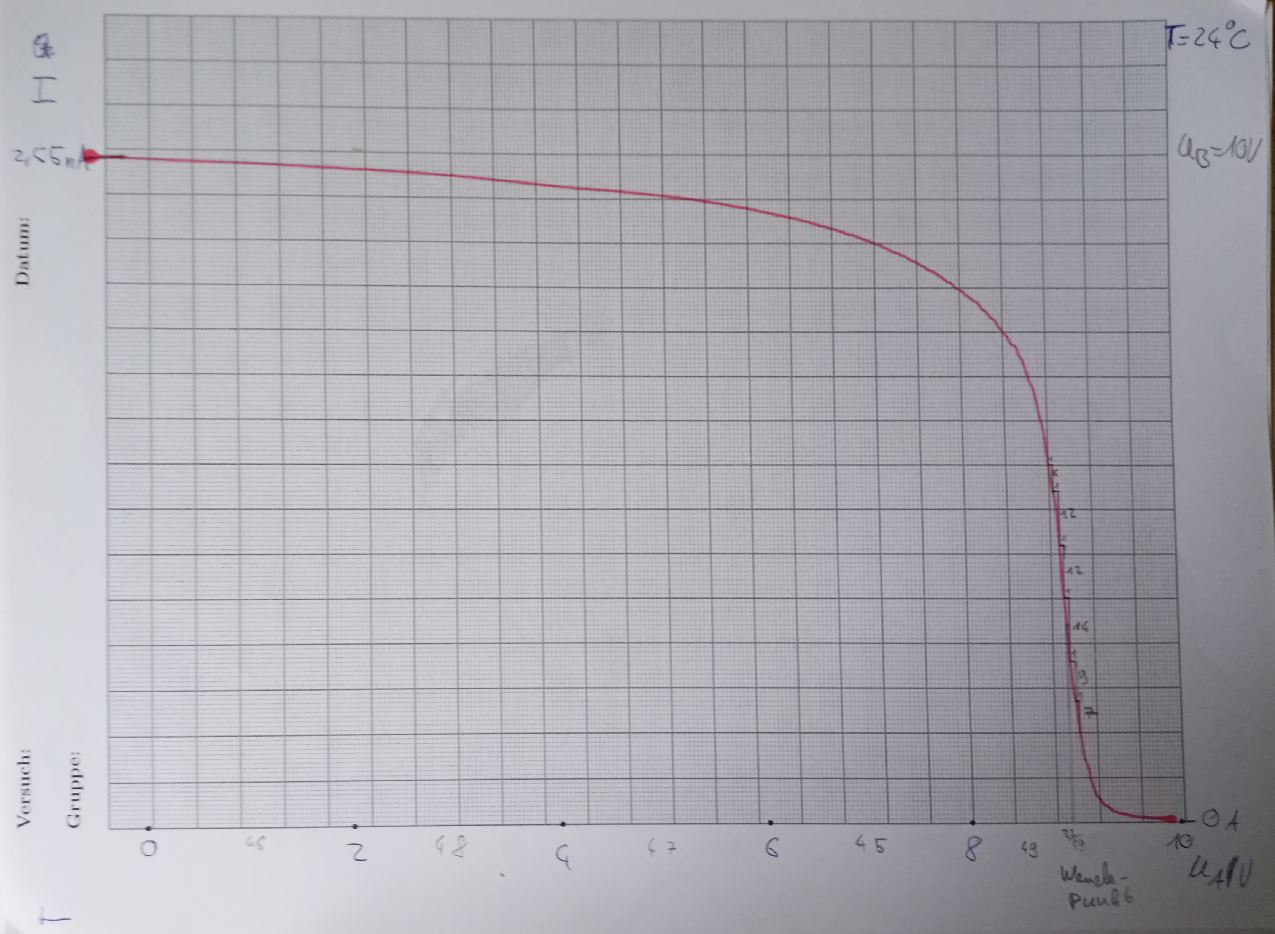
\includegraphics[width=\textwidth]{Abbildungen/v601_A.pdf}
    \caption{Die Ergebnisse der Messung A.}
    \label{fig:messung_a}
\end{figure}

\noindent
Aus der integralen Energieverteilung der Elektronen in Messung A kann auf die Geschwindigkeitsverteilung
bzw die differenzielle Energieverteilung geschlossen werden.
In Messung A haben die meisten Elektronen eine Energie entsprechend der \qty{8.94}{\volt} effektiver Beschleunigungsspannung.
In Messung B beschreibt die integrale Energieverteilung im Bereich \qty{0}{\volt} bis \qty{4}{\volt} einen Linear abfallenden Zusammenhang.
Bei Bremsspannungen größer als 4 Volt zeigt das Messgerät einen negativen Strom an, was hier als Fehler des Messgerätes interpretiert wird.
Die Form der Kurve flacht in diesem Bereich auch deutlich ab.
Die Energieverteilung der Elektronen ist demnach im Bereich 0 bis 4 \unit{\volt} gleichmäßig hoch und ist in einem Bereich größer als
\qty{4}{\volt} nahe der null.

\subsection{Auswertung der Franck-Hertz-Kurve}
Um das Energieniveau der Übergänge in den Hg-Atomen zu messen werden die Maxima der Franck-Hertz-Kurve in den Messungen C und D
ausgewertet.
Zunächst werden per Hand die Maxima der Kurve auf dem Millimeterpapier bestimmt und die Abstände $N_\text{dist}$ zwischen den
Maxima notiert.
Um die Abstände der Maxima in Einheiten von $U_B$ umzurechnen werden auch die Abstände der Skalenpunkte $N_\text{scale}$ notiert.
Um den Effekt von von möglichen Mess- und Ablesefehlern klein zu halten und die Abweichungen einzuschätzen wird von beiden Größen 
das Arithmetische Mittel $\overline{x}$ sowie die Standartabweichung $\sigma(x)$ berechnet.
Der reale Spannungsunterschied zwischen den Maxima $U_{1}$ berechnet sich durch
\begin{align}
    U_{1} = \frac{N_\text{dist}}{N_\text{scale}}\cdot \qty{5}{\volt}
\end{align}
Um den Messfehler von $U_{1}$ richtig einzuschätzen werden die Regeln der Gaußschen Fehlerfortpflanzung verwendet.
\begin{align}
    \sigma\left(U_{1}\right) = \sqrt{\left(\frac{\partial U_{1}}{\partial N_\text{dist}} \cdot \sigma\left(N_\text{dist}\right) \right)^2%
                                                    +  \left(\frac{\partial U_{1}}{\partial N_\text{scale}} \cdot \sigma\left(N_\text{scale}\right) \right)^2 }
\end{align}

\subsubsection{Auswertung der Messungen}
\textbf{Bild einfügen }
Bei der Messung D war es für die höchsten beiden Peaks nicht möglich die Extremstellen eindeutig zu bestimmen.
Deshalb werden diese Extremstellen für die Berechnung der Anregungsenergie nicht berücksichtigt.
\begin{table}
    \begin{minipage}{0.5\textwidth}
        \centering
        \begin{tabular}{S S}
            \toprule
            {$N_\text{dist}$} & {$N_\text{scale}$} \\
            \midrule
            34 & 36 \\
            36 & 38 \\
            36 & 35 \\
            37 & 37 \\
            38 & 37 \\
            & 37 \\
            \bottomrule
        \end{tabular}
        \caption{Ergebnisse Messung C}
    \end{minipage}%
    \begin{minipage}{0.5\textwidth}
        \centering
        \begin{tabular}{S S}
            \toprule
            {$N_\text{dist}$} & {$N_\text{scale}$}  \\
            \midrule
            19 & 19 \\
            18 & 23 \\
            20 & 21 \\
            20 & 20 \\
            19 & 18 \\
            21 & 21 \\
               & 20 \\
            \bottomrule
        \end{tabular}
        \caption{Ergebnisse Messung D}
    \end{minipage}
\end{table}

\noindent
Aus den ermittelten Werten ergibt sich in Versuch C ergeben sich für die Skalenlänge ein Wert von
$N_\text{scale, C} = \num{36.7 +- 0.9}$ und für den Abstand der Peaks ein Wert von $N_\text{dist,C} = \num{36.2 +- 1.3}$.
Daraus berechnet sich ein Abstand von $U_{1,C} = \qty{4.94 +- 0.22}{\volt}$. 
In Versuch D ergibt sich aus den Werten $N_\text{scale, D} = \num{20.3 +- 1.5}$ und $N_\text{dist, D} = \num{19.5}$
ein Abstand von $U_{1,D} = \qty{4.8 +- 0.4}{\volt}$.

\subsubsection{Berechnung der emittierten Wellenlänge}
Nach der Formel (\textbf{Referenz}) wird die Wellenlänge der emittierten Strahlung gemessen.
\begin{align}
    \lambda = \frac{c}{\nu} = \frac{c \cdot h}{e_0 \cdot U_1}
\end{align}
Mit den Werten $h=\qty{6.62607015e-34}{\joule\s}$, $e_0 = \qty{1.602176634e-19}{\C}$ 
und $c = \qty{299792458.0}{\meter\per\second}$ (vgl. \cite{scipy})
ergeben sich für die jeweiligen Messungen Wellenlängen von $\lambda_C = \qty{ 2.51 +- 0.11 e-07}{\m}$ und $\lambda_D= \qty{2.58 +- 0.23 e-07}{\m}$.